\documentclass[10pt]{article}
\usepackage[polish]{babel}
\usepackage[utf8]{inputenc}
\usepackage[T1]{fontenc}
\usepackage{amsmath}
\usepackage{amsfonts}
\usepackage{amssymb}
\usepackage[version=4]{mhchem}
\usepackage{stmaryrd}
\usepackage{graphicx}
\usepackage[export]{adjustbox}
\graphicspath{ {./images/} }

\title{LIGA MATEMATYCZNA \\
 im. Zdzisława Matuskiego \\
 PÓŁFINAŁ \\
 29 lutego 2016 \\
 GIMNAZJUM }

\author{}
\date{}


\newcommand\varangle{\mathop{\sphericalangle}}

\begin{document}
\maketitle
\section*{ZADANIE 1.}
Dany jest czworokąt wypukły \(A B C D\), gdzie \(\varangle C B A=60^{\circ}, \varangle D B A=50^{\circ}, \varangle B A C=60^{\circ}\), \(\varangle C A D=20^{\circ}\). Wyznacz miare kata \(\varangle A C D\).\\
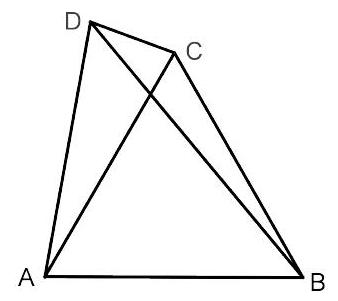
\includegraphics[max width=\textwidth, center]{2024_11_21_dc6490e81fa2cf87933ag-1}

\section*{ZADANIE 2.}
Uzasadnij, że dla dowolnej liczby naturalnej \(n\) liczba

\[
\frac{(n+2015)(n+2016)}{2}
\]

jest naturalna.

\section*{ZADANIE 3.}
Suma cyfr pewnej liczby trzycyfrowej jest równa 11. Jeżeli przestawimy cyfry jedności i setek, nie zmieniając cyfry dziesiątek, to otrzymamy liczbę o 99 mniejszą. Wyznacz wszystkie takie liczby trzycyfrowe.

\section*{ZADANIE 4.}
Wykaż, że dla dowolnej liczby naturalnej \(n\) liczba

\[
11 \ldots 122 \ldots 233 \ldots 344 \ldots 4
\]

jest podzielna przez 12, gdy jedynek jest \(n\), dwójek jest \(2 n\), trójek jest \(3 n\), czwórek jest \(4 n\).

\section*{ZADANIE 5.}
Odcinek \(B C\) jest średnicą okręgu oraz \(|B C|=\sqrt{901},|B D|=1,|D A|=16\). Niech \(|E C|=x\). Oblicz \(x\).\\
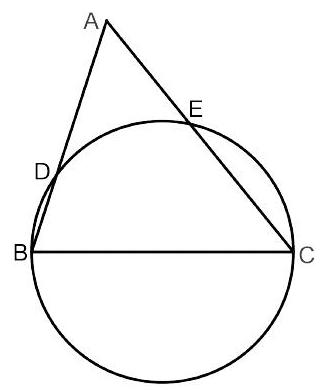
\includegraphics[max width=\textwidth, center]{2024_11_21_dc6490e81fa2cf87933ag-1(1)}


\end{document}